\def \currentAuthor {Gabi Sorglos} %so kann jederzeit der Autor geändert werden -> wird in der Fusszeile angezeigt.

\chapter*{Einleitende Bemerkungen}

\chapter*{Notationen}
Beschreibung wie Code, Hinweise, Zitate etc. formatiert werden  


\chapter{Projektmanagement}
%todo: Projektmanagementscheiße bullshitten
\section{Metainformationen}
\subsection{Team}
\subsection{Betreuer}
\subsection{Partner}
\subsection{Ansprechpartner}
\section{Vorerhebungen}
\subsection{Projektzieleplan}


\newpage
\subsection{Projektumfeld}
\begin{itemize}
	\item Identifikation der Stakeholder
	\item Charakterisierung der Stakeholder
	\item Maßnahmen
	\item Grafische Darstellung des Umfeldes
\end{itemize}
\subsection{Risikoanalyse}
\subsubsection{Risikoidentifikation}
Folgende Risiken können während der Projektdurchführung erwartet werden:
\begin{itemize}
	\item[\textbf{R1}] Projektmitglied steig aus dem Projekt aus.
	\item[\textbf{R2}] Projektpartner stellt seine Kooperation ein.
	\item[\textbf{R3}] Projektpartner ändert seine Anforderungen.
	\item[\textbf{R4}] Termine können nicht eingehalten werden.
	\item[\textbf{R5}] Anforderungen werden nicht erreicht.			
\end{itemize}

\subsubsection{Bewertung und Behandlung}
Die aufgelisteten Risiken werden nach Auswirkung und Eintrittswahrscheinlichkeit bewertet.
Je höher die Zahl in der Tabelle, desto höher ist die Auswirkung bzw. Einwirkung.
\begin{table}[h]
	\begin{tabular}{l|c|c}
		\textbf{Risiko}                           & \multicolumn{1}{l|}{\textbf{Wahrscheinlichkeit}} & \multicolumn{1}{l}{\textbf{Auswirkung}} \\ \hline
		\textbf{R1} Ausstieg Projektmitglied                  & 3                                                & 10                                      \\
		\textbf{R2} Projektpartner stellt Kooperation ein     & 2                                                & 10                                      \\
		\textbf{R3} Projektpartner ändert seine Anforderungen & 4                                                & 7                                       \\
		\textbf{R4} Termine können nicht eingehalten werden   & 3                                                & 6                                       \\
		\textbf{R5} Anforderungen werden nicht erreicht       & 2                                                & 8                                      
	\end{tabular}
	\caption{Analyse Einwirkung \& Auswirkung}
	\label{Abb_Einwirkung_Auswirkung}
\end{table}
\newpage

\subsubsection{Risikomatrix}
\begin{figure}[h]
	\centering
	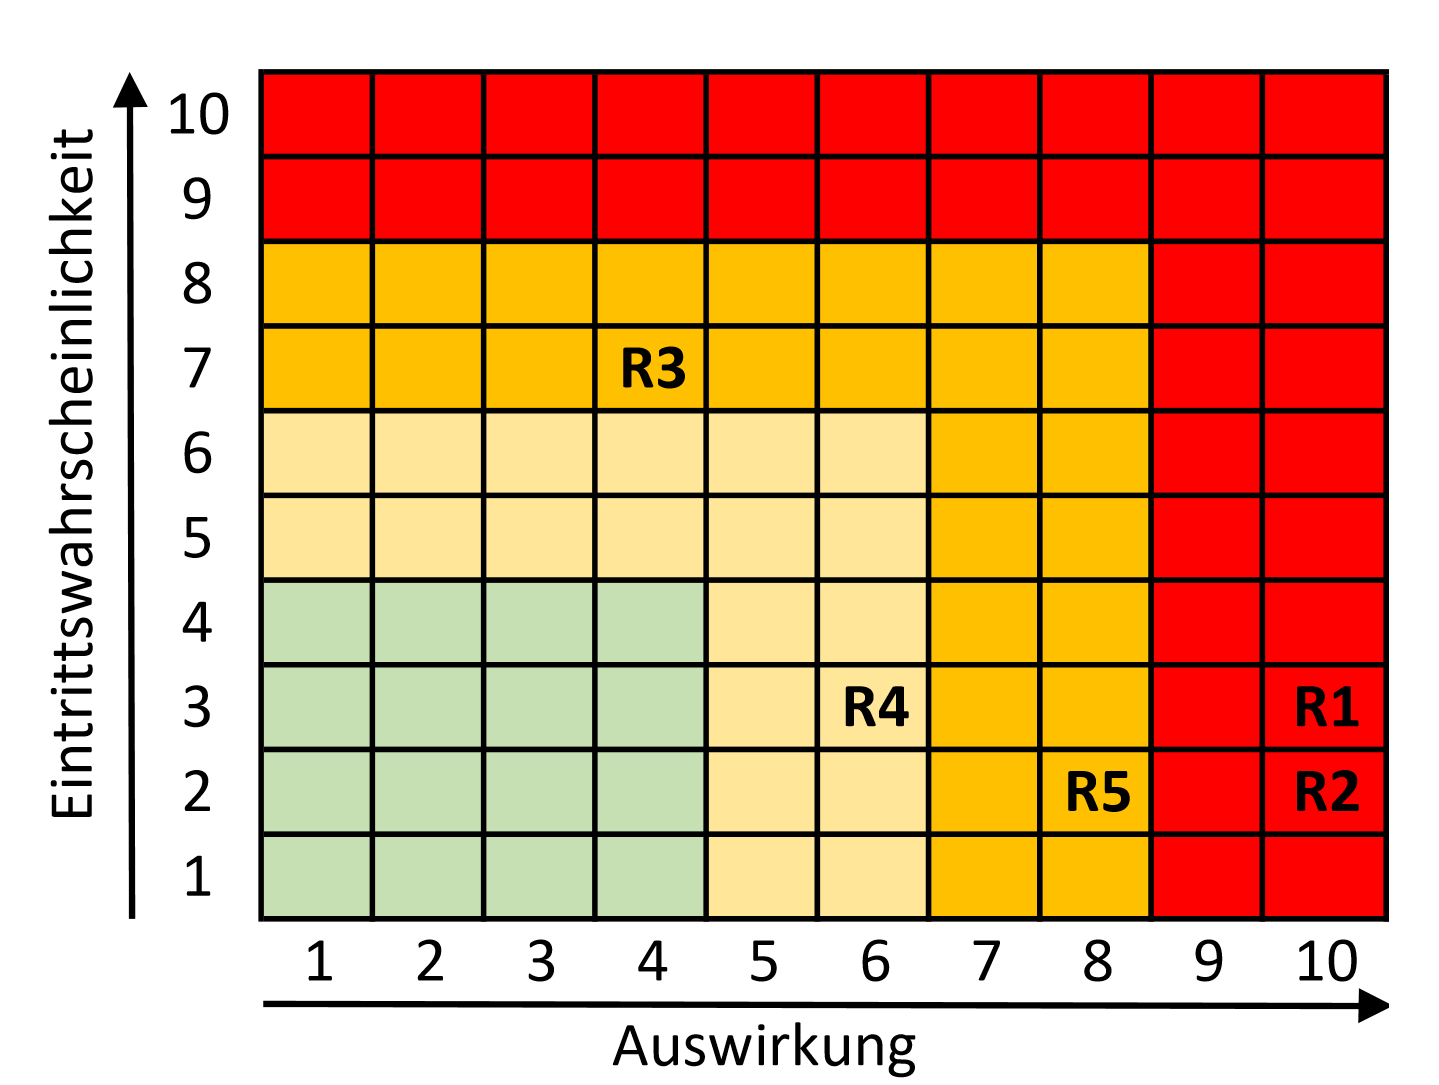
\includegraphics[scale=0.6]{figures/matrix.png}
	\caption{Risikomatrix}
	\label{Abb_Risikomatrix}
\end{figure}


\newpage
\section{Pflichtenheft}
\subsection{Zielbestimmung}
\section{IST Zustand}
IT-ManagerInnen an Tirols Schulen können Probleme mit der Infrastruktur melden und Anfragen zur Beschaffung von Ressourcen/Komponenten stellen.
\\
Sie können den Bearbeitungsverlauf ihrer Tickets beobachten. SystembetreuerInnen empfangen die Tickets der IT-ManagerInnen, welche sich in ihrem Cluster befinden. SystembetreuerInnen bearbeiten die Tickets und antworten auf die Anfragen.

\begin{figure}[h]
	\centering
	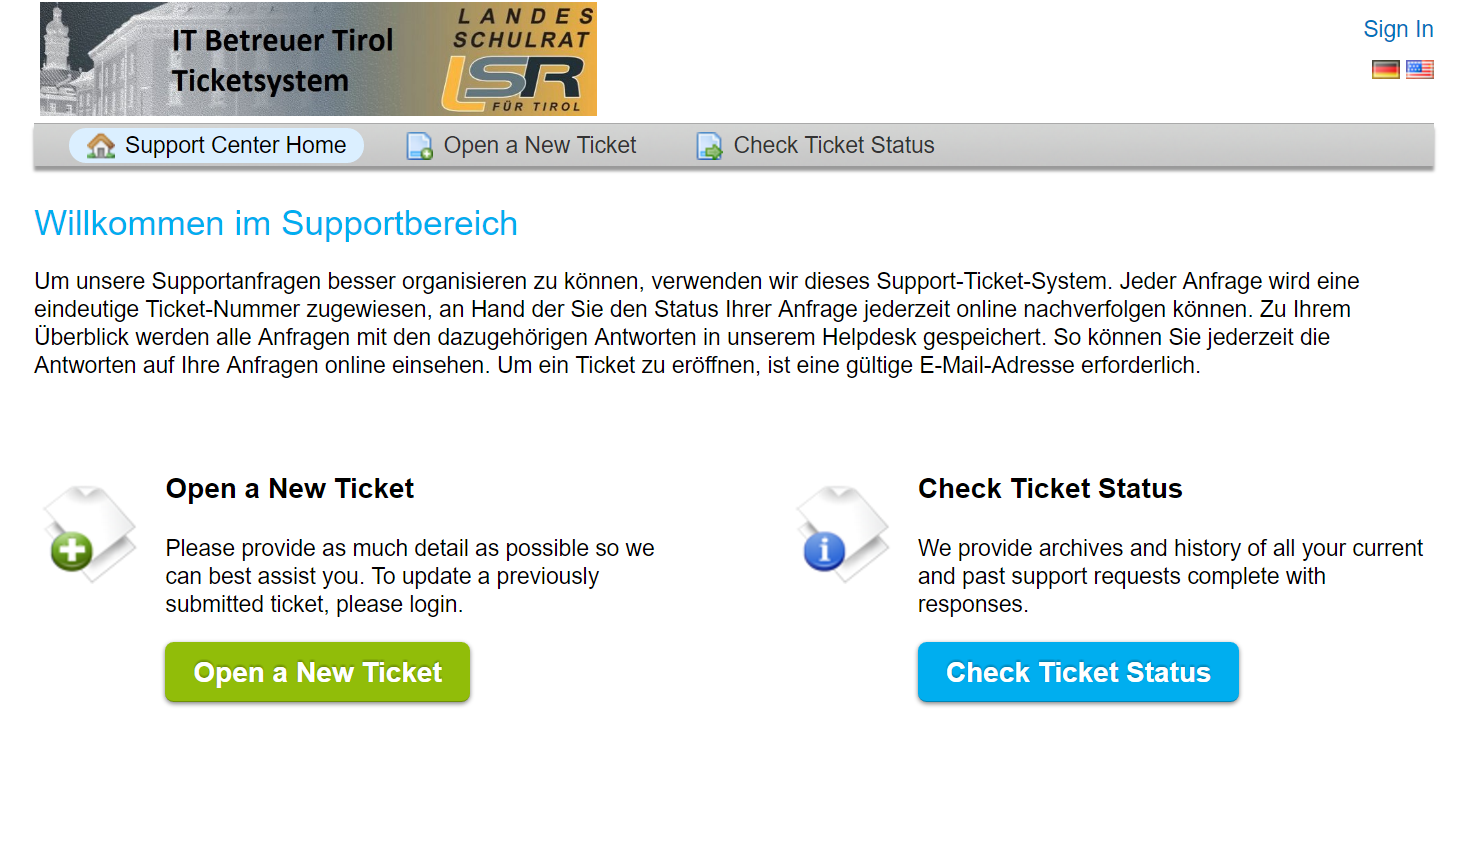
\includegraphics[scale=0.725]{figures/Ist_Login.png}
	\caption{IST-Zustand OS-Ticket}
	\label{Abb_IST-Zustand}
\end{figure}
\noindent Die Benutzerschnittstelle ist derzeit nur auf die Benutzung mit großen Bildschirmen (ab 1024 Pixel Bildschirmbreite) ausgelegt. Sie kann sich nicht an kleinere Formate (Smartphone, etc.) anpassen.

\section{SOLL Zustand}
Bessere Usability soll mit Hilfe von Mobile-First Orientierung auf Basis von Bootstrap erreicht und wenn möglich die Ticketerstellung vereinfacht werden.
\\
Das Backend soll die Aufteilung in mehrere hierarchische Organisationseinheiten ermöglichen und eine Erweiterung von Landesebene auf Bundesebene zulassen. Des Weiteren gilt es, den AnwenderInnen den Ticketingprozess intuitiver zu gestalten.

\subsection{SMART}
\begin{description}
	\item[S] Spezifisch\newline
	Systembetreuer und IT-Manager können Support- und Beschaffungsanfragen mit Hilfe des Ticketsystems abwickeln.
	\item[M] Messbar\newline
	Systembetreuer empfangen die Tickets und kümmern sich um die Probleme. Die Schulen werden in Cluster eingeteilt und von Systembetreuern verwaltet. 
	\item[A] Attraktiv\newline
	Die Plattform muss auf jedem Endgerät verfügbar sein (Responsive Design). Das Absetzen und Ansehen von Tickets soll vereinfacht werden, die Plattform bietet einige Funktionen die für das System relevant sind.
	\item[R] Realisierbar\newline
	Zum Realisieren wird eine Testumgebung von Seiten des Betreuers zur Verfügung gestellt. Das Responsive Design wird mithilfe eines Framework (Bootstrap) realisiert.
	\item[T] Terminisierbar\newline
	Im Juni 2017 wird das Projekt abgeschlossen und eine technische Dokumentation des Projekts liegt vor.
\end{description}


\subsection{Produkteinsatz und Umgebung}
%--------------------------------
%todo: Anwender des Systems beschreiben (steht auch so in der Vorlage)
%--------------------------------
\subsection{Projektumfeldanalyse}
\subsubsection{Einflussfaktoren}
Das Projekt wurde durch den Landesschulrat Tirol in Auftrag gegeben. Die Ansprechperson, Herr Helmut Hammerl, informiert uns über den IST und SOLL-Zustand der Plattform und unterstützt das Projekt mit Ideen und Hilfestellungen bei Problemstellungen.
\\
Des Weiteren beeinflussen die Anwender (IT-Manager) und die Systembetreuer der Plattform das Projektresultat. Da auf die Anwenderfreundlichkeit viel Wert gelegt wird, spielen diese Faktoren eine wirkliche Rolle.
\\
Die Projektbetreuer Stefan Stolz und Alexander Scharmer sind für auftretende Fragen, bezüglich Problemstellungen die während des Projekts auftreten können, enorm einflussreich.
\newpage
\subsection{Stakeholder}
\subsubsection{Stakeholder Identifizieren}
\begin{table}[h]
	\centering
	\begin{tabular}{|lll|}
		\hline
		Stakeholder          & Einfluss &  Konfliktpotential      \\ \hline                         
		Mag. Helmut Hammerle & 3         & 0                  \\ 
		Dr. Stefan Walch     & 2         & 0                  \\
		Stefan Stolz         & 1         & +                  \\ 
		Alexander Scharmer   & 1         & +                  \\ 
		Michael Gamper       & 0         & 0                  \\ 
		LSI DI Anton Lendl   & 3         & 0                  \\ 
		Team Mitglieder      & 2         & 0                   \\ \hline			
	\end{tabular}
	\caption{Stakeholder Identifikation}
	\label{Tbl_Stakeholder_Identifikation}
\end{table}


\subsubsection{Stakeholder Klassifizieren}	

%todo: Formatierung der Tabelle
\begin{table}[h]
	\centering
	\begin{tabular}{|lll|}
		\hline
		Stakeholder          & Risiken durch Stakeholder                        & Strategien                                            \\ \hline
		Mag. Helmut Hammerl & Ändern der Ansprüche          & Unterschriebenes Pflichtenheft  \\
		Dr. Stefan Walch      & Nicht bestätigen des Projektantrages             & Durchdachter Projektantrag                            \\
		Stefan Stolz         & falsche Informationen, kein Interesse & regelmäßiges Treffen             \\
		Alexander Scharmer   & falsche Informationen, kein Interesse & regelmäßiges Treffen              \\
		Michael Gamper       & Nicht bestätigen des Projektantrages             & Durchdachter Projektantrag                            \\
		LSI DI Anton Lendl   & Nicht bestätigen des Projektantrages             & Durchdachter Projektantrag                            \\
		Team Mitglieder      & Mangelnde Motivation                             & Faire Arbeitsverteilung           \\ \hline			
	\end{tabular}
	\caption{Stakehodler Klassifikation}
	\label{Tbl_Stakeholder_Klassifikation}
\end{table}


\subsection{Funktionalitäten}
\subsection{Muss Anforderungen}
IT-ManagerInnen und Systembetreuer müssen sich unter itsys-tirol.at, einem Portal des Landesschulrates, basierend auf OSticket anmelden können. Des Weiteren sollen die Schulen selbst bestimmen, wer einen Zugang zum Portal erhalten soll, um Tickets erstellen zu können.
\\
Die angemeldeten IT-ManagerInnen müssen Probleme mit der Infrastruktur melden können und Anfragen zur Beschaffung von Ressourcen bzw. Komponenten einreichen können.
\\
SystembetreuerInnen müssen die Tickets der IT-ManagerInnen empfangen, welche sich in ihrem Cluster befinden. Die eingereichten Tickets sollen von den Systembetreuern bearbeitet werden können.

\subsection{Soll Anforderungen}
Es soll eine neue Weboberfläche entwickelt werden, die auf dem HTML \& CSS Framework Bootstrap basiert. Dieses soll sich auf Einfachheit in der Anwendung und Benutzerfreundlichkeit fokussieren. Die Latenzzeit sollte so niedrig wie möglich gehalten werden um ein Reibungsloses Arbeiten zu ermöglichen.

%todo: Testfälle sind furchtbar und müssen generell nocheinmal überarbeitet werden
\subsection{Testszenarien und Testfälle}
Die Testfälle in unserem Projekt beziehen sich auf das Ticketingsystem OSTicket.

\section{Testfälle}
\subsection{Testfall A}
\begin{itemize}
	\item \textbf{Beschreibung:} Ein IT-Manager möchte ein Ticket erstellen.
	\item \textbf{Vorbedingung:} Der User benötigt ein internetfähiges Gerät und muss im Portal eingeloggt sein.
	\item \textbf{Aktion:} Der Benutzer wählt den Tab "Neues Ticket" und füllt die notwendigen Felder aus.
	\item \textbf{Soll-Reaktion:} Das System setzt das Ticket für den zuständigen Systembetreuer sichtbar.
\end{itemize}
Tester:
\\M
Datum:

\subsection{Testfall B}
\begin{itemize}
	\item \textbf{Beschreibung:} Ein Systembetreuer möchte ein Ticket bearbeiten.
	\item \textbf{Vorbedingung:} Der Systembetreuer benötigt ein internetfähiges Gerät und muss im Portal eingeloggt sein.
	\item \textbf{Aktion:} Der Systembetreuer wählt den Tab "Meine Tickets" und wählt ein Ticket aus das Bearbeitet werden muss. Durch die Beschreibung des Tickets, weiß der Systembetreuer über die Problemstellung Bescheid und kann dementsprechend handeln.
	\item \textbf{Soll-Reaktion:} Der Systembetreuer kann sich um die Problemstellung kümmern und das Ticket nach erfolgreicher Bearbeitung wieder schließen.
\end{itemize}
Tester:
\\
Datum:

\subsection{Testfall C}
\begin{itemize}
	\item \textbf{Beschreibung:} Ein Anwender möchte ein bestimmtes Ticket suchen und dieses begutachten. 
	\item \textbf{Vorbedingung:} Der Anwender benötigt ein internetfähiges Gerät und muss im Portal eingeloggt sein.
	\item \textbf{Aktion:} Der Anwender gibt im Suchfeld ein Stichwort ein nach dem er suchen möchte. 
	\item \textbf{Soll-Reaktion:} Das gesuchte Ticket soll angezeigt werden.
\end{itemize}
Tester:
\\
Datum:



\subsection{Liefervereinbarung}
\begin{itemize}
	\item Lieferumfang
	\item Modus
	\item Verteilung(Deployment)
\end{itemize}

%todo: viel Bullshitten
\section{Planung}
\subsection{Projektstrukturplan}
\subsection{Meilensteine}
\subsection{Gant-Chart}
\subsection{Abnahmekriterien}
\subsection{Pläne zur Evaluierung}
\subsection{Ergänzungen und zu klärende Punkte}

\chapter{Vorstellung des Produktes}
In diesem Kapitel werden die einzelnen Ansätze aufgelistet und evaluiert, die während des Projekts durchprobiert wurden.
\section{Realisierbarkeit OSTicket}
OSTicket hat sich als umfangreicher herausgestellt wie zu Beginn des Projekts angenommen wurde. Nach Ausarbeitung des konzeptuellen Ziels des Projektes erfolgte eine lange Phase der Evaluation, Einarbeitung und Dokumentation von OSTicket. Nach ca. 30 Stunden dieser Phase, in der die Komplexität und Schwerfälligkeit des Systems OSTicket langsam zu Tage gefördert wurde. Die Anzahl der Dateien setzt sich folgendermaßen zusammen:
\begin{itemize}
	\item 414 .php Dateien
	\item 15 .css Dateien
	\item 9 .less Dateien
	\item 61 .sql Dateien
	\item 1 .html Datei
	\item \textbf{Ges. 500 Dateien}
\end{itemize}

Ein weiteres Hindernis ergibt sich durch die Absenz einer auch nur annähernd aktuellen Dokumentation des laufend erweiterten und angepassten OSTicket.
\\
Um die Realisierbarkeit zu veranschaulichen nun einige Codeauszüge aus OSTicket.
\subsection{Codebeispiele}
\begin{lstlisting}[language=PHP, caption=Auszug aus osTicket, label=code:qj]
<?php
/**************************************************
main.inc.php

Master include file which must be included at the 
start of every file.
The brain of the whole sytem. Don't monkey with it.

Peter Rotich <peter@osticket.com>
Copyright (c)  2006-2013 osTicket
http://www.osticket.com

Released under the GNU General Public License WITHOUT
 ANY WARRANTY.
See LICENSE.TXT for details.

vim: expandtab sw=4 ts=4 sts=4:
***************************************************/

#Disable direct access.
if(isset($_SERVER['SCRIPT_NAME'])
&& !strcasecmp(basename($_SERVER['SCRIPT_NAME'])
,basename(__FILE__)))
die('kwaheri rafiki!');

require('bootstrap.php');
Bootstrap::loadConfig();
Bootstrap::defineTables(TABLE_PREFIX);
Bootstrap::i18n_prep();
Bootstrap::loadCode();
Bootstrap::connect();

#Global override
$_SERVER['REMOTE_ADDR'] = osTicket::get_client_ip();

if(!($ost=osTicket::start()) || !($cfg = $ost->getConfig()))
Bootstrap::croak(__('Unable to load config info 
from DB. Get tech support.'));

//Init
$session = $ost->getSession();

//System defaults we might want to make global//
#pagenation default - user can override it!
define('DEFAULT_PAGE_LIMIT', $cfg->getPageSize()?$cfg->getPageSize():25);

#Cleanup magic quotes crap.
if(function_exists('get_magic_quotes_gpc') && get_magic_quotes_gpc()) {
$_POST=Format::strip_slashes($_POST);
$_GET=Format::strip_slashes($_GET);
$_REQUEST=Format::strip_slashes($_REQUEST);
}

// extract system messages
$errors = array();
$msg=$warn=$sysnotice='';
if ($_SESSION['::sysmsgs']) {
extract($_SESSION['::sysmsgs']);
unset($_SESSION['::sysmsgs']);
}
?>

\end{lstlisting}
%todo: Zitate (Codezitate des Programmierers, Netzer fragen)
%todo: wie genau soll man den begründen das da Code a scheiß is?
In diesem Codeauszug wird die Komplexität von osTicket sehr gut veranschaulicht, der Aufruf von elf statischen Funktionen und der dürftigen Dokumentation der Programmierer "Don't monkey around with it", machen den Code unlesbar.






%----------------------------------------------
\section{Systemdokumentation}
%todo: Systemdokumentation aus SYP hinzufügen, ist jedoch nicht ganz so einfach da Probleme mit Packages auftreten 


%-------------------------------------
%todo: Formatierungschaos im Chapter Problemanalyse beheben und Inhalt überarbeiten
%-------------------------------------

\chapter{Problemanalyse}

\section{USE-Case-Analyse}
{\linespread{.5}
	\textbf{Akteure:}
	\begin{itemize}
		\item Systembetreuer
		\item Anwender (IT-Manager und eventuell Lehrer, in Folgendem Anwender genannt)
\end{itemize}}

\vspace{-.5cm}
\begin{table}[h]
	\centering
	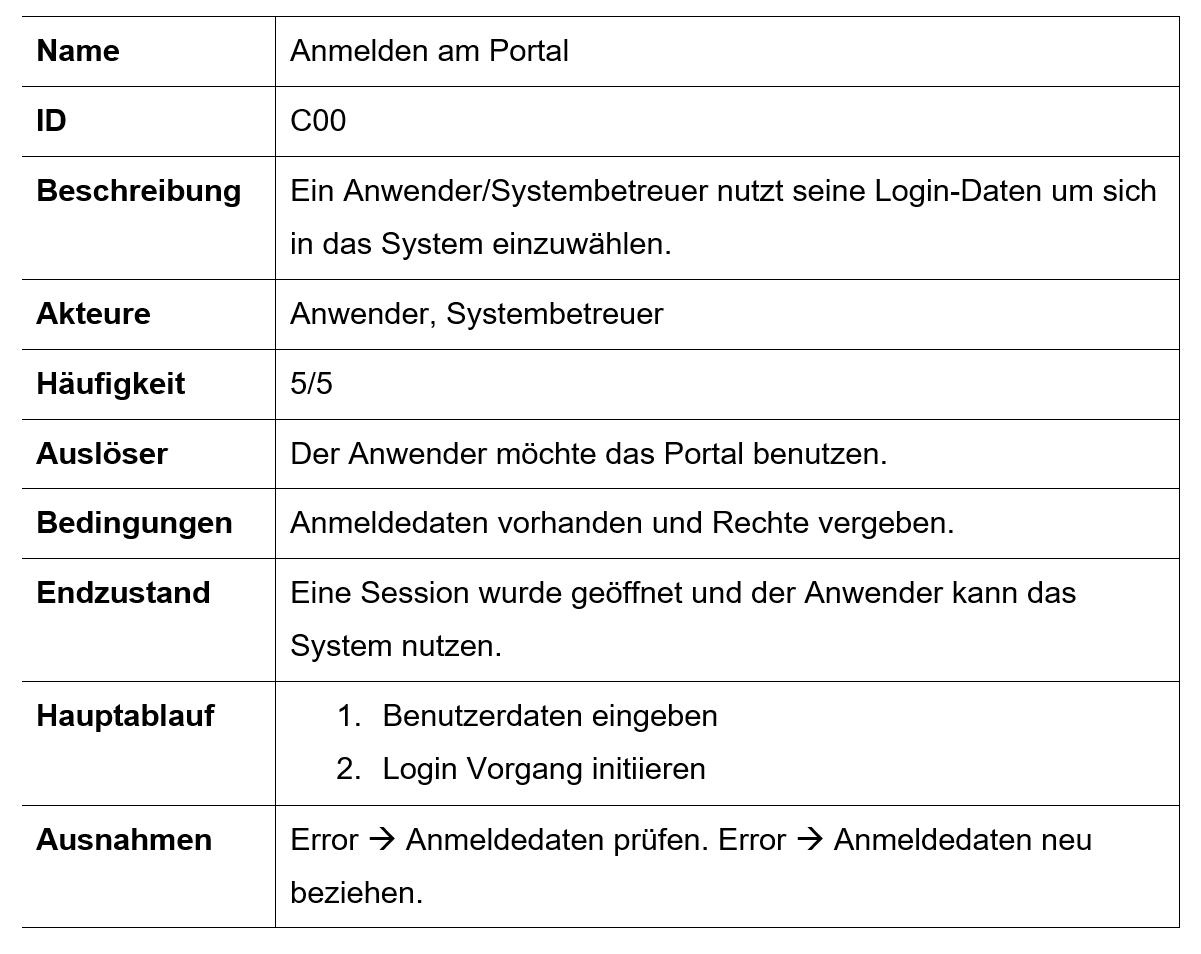
\includegraphics[scale=0.51]{figures/C00.png}
	\caption{Use-Case C00}
	\label{Abb_C00}
\end{table}
\newpage
\vspace{-.5cm}	
\begin{table}[h]
	\centering
	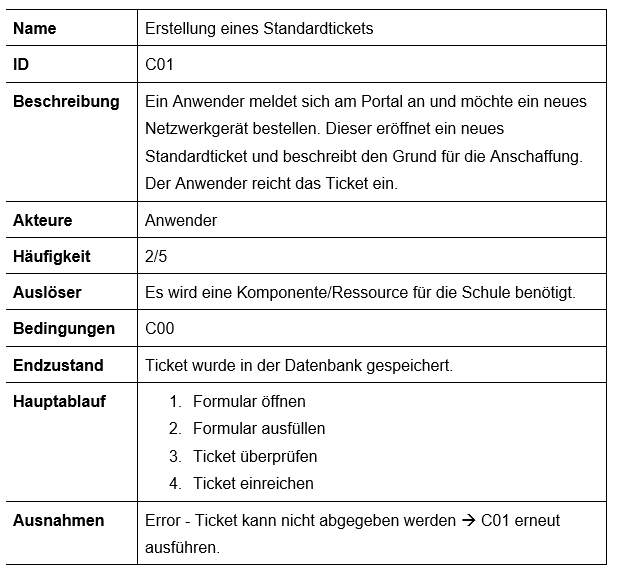
\includegraphics[scale=0.55]{figures/C01.png}
	\caption{Use-Case C01}
	\label{Abb_C01}
\end{table}
\newpage
\vspace{-.5cm}	
\begin{table}[h]
	\centering
	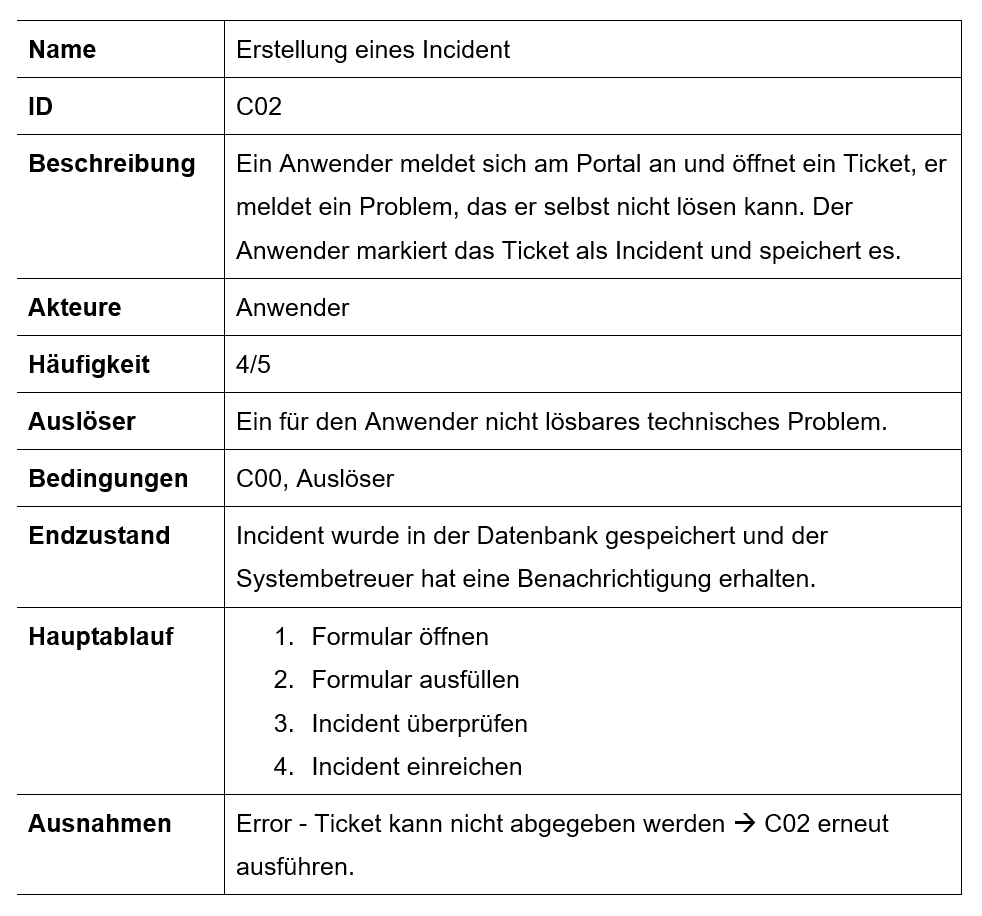
\includegraphics[scale=0.6]{figures/C02.png}
	\caption{Use-Case C02}
	\label{Abb_C02}
\end{table}

\vspace{-.5cm}	
\begin{table}[h]
	\centering
	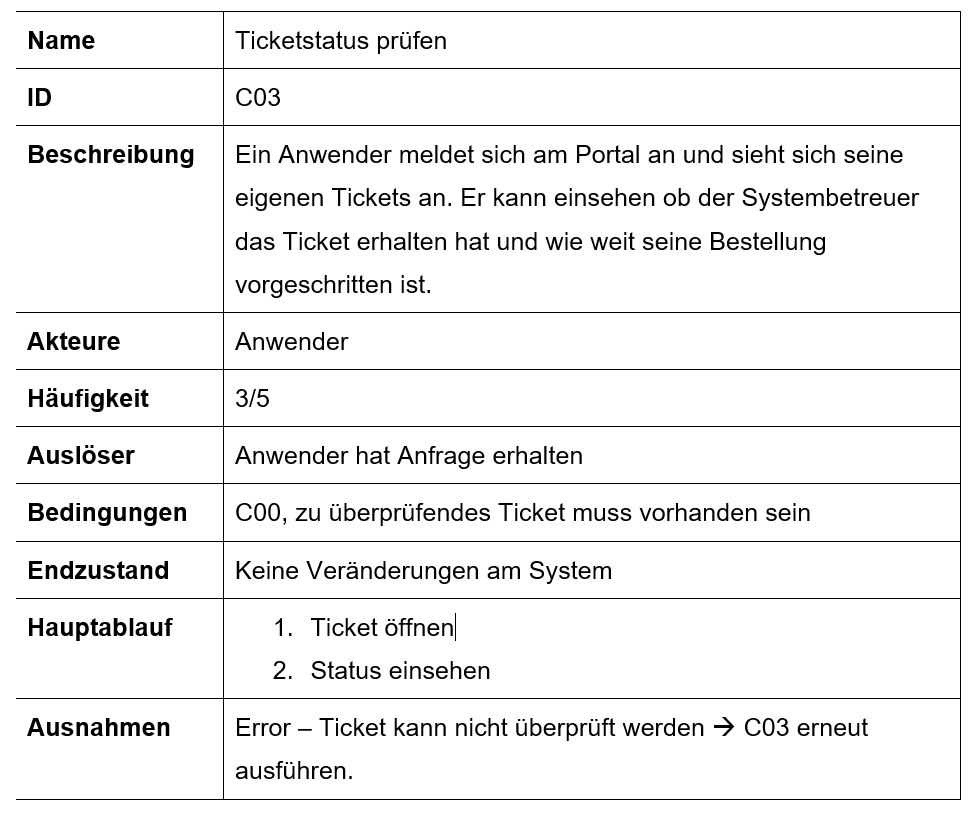
\includegraphics[scale=0.62]{figures/C03.png}
	\caption{Use-Case C03}
	\label{Abb_C03}
\end{table}
\newpage
\vspace{-.5cm}	
\begin{table}[h]
	\centering
	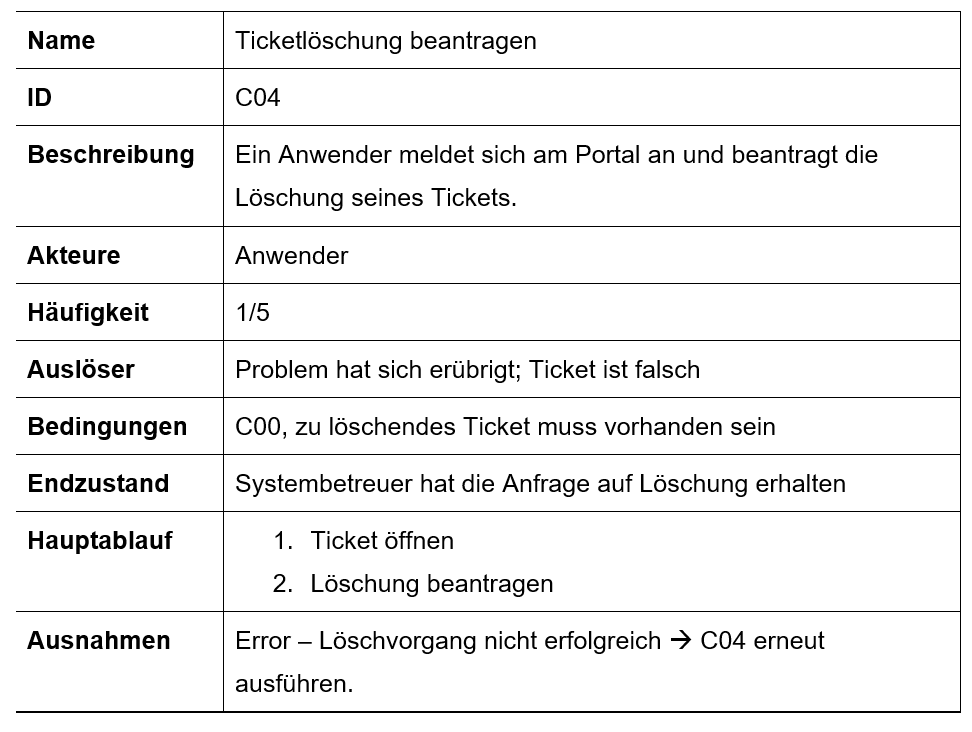
\includegraphics[scale=0.62]{figures/C04.png}
	\caption{Use-Case C04}
	\label{Abb_C04}
\end{table}


\vspace{-.5cm}	
\begin{table}[h]
	\centering
	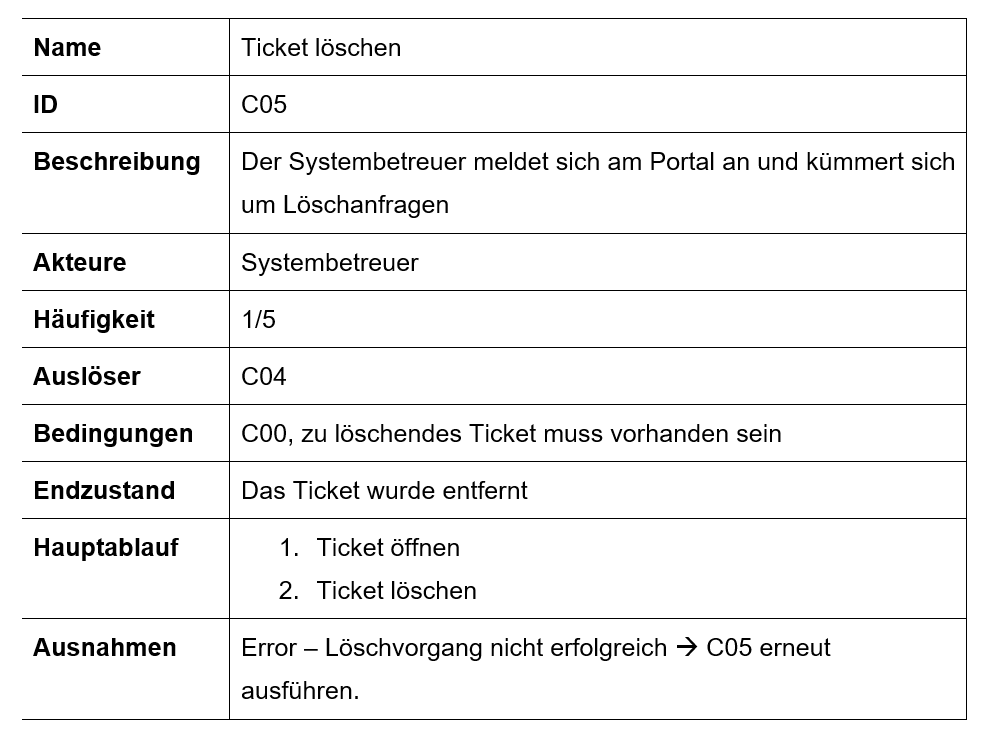
\includegraphics[scale=0.62]{figures/C05.png}
	\caption{Use-Case C05}
	\label{Abb_C05}
\end{table}
\newpage
\vspace{-.5cm}	
\begin{table}[h]
	\centering
	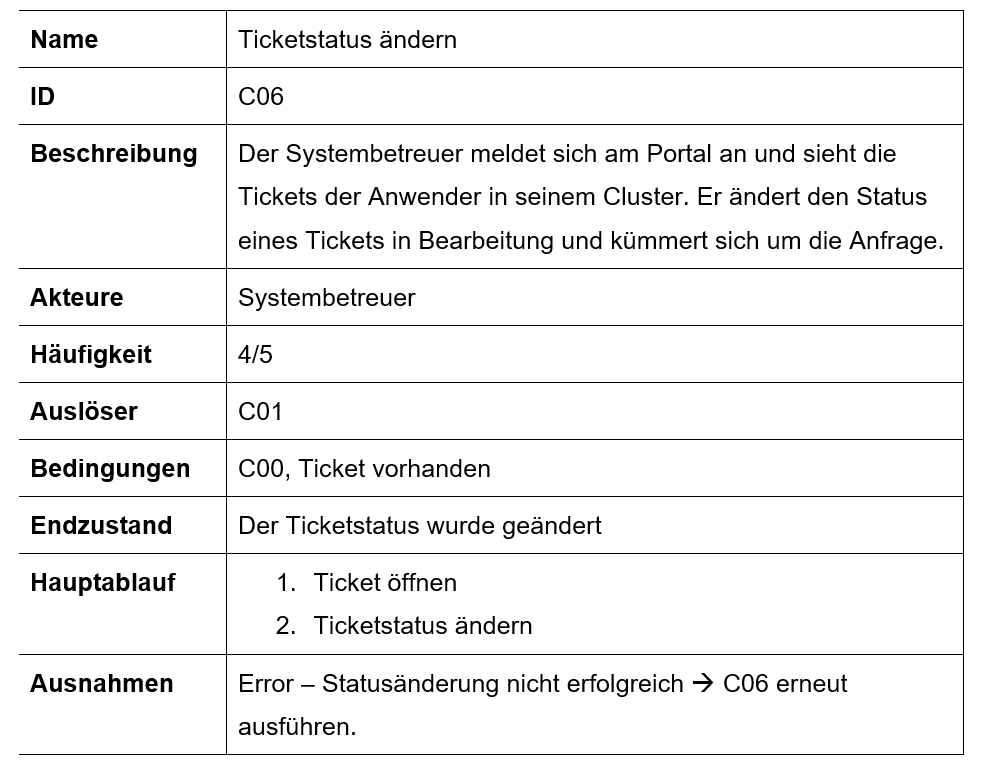
\includegraphics[scale=0.62]{figures/C06.png}
	\caption{Use-Case C06}
	\label{Abb_C06}
\end{table}
\newpage
\vspace{-.5cm}	
\begin{table}[h]
	\centering
	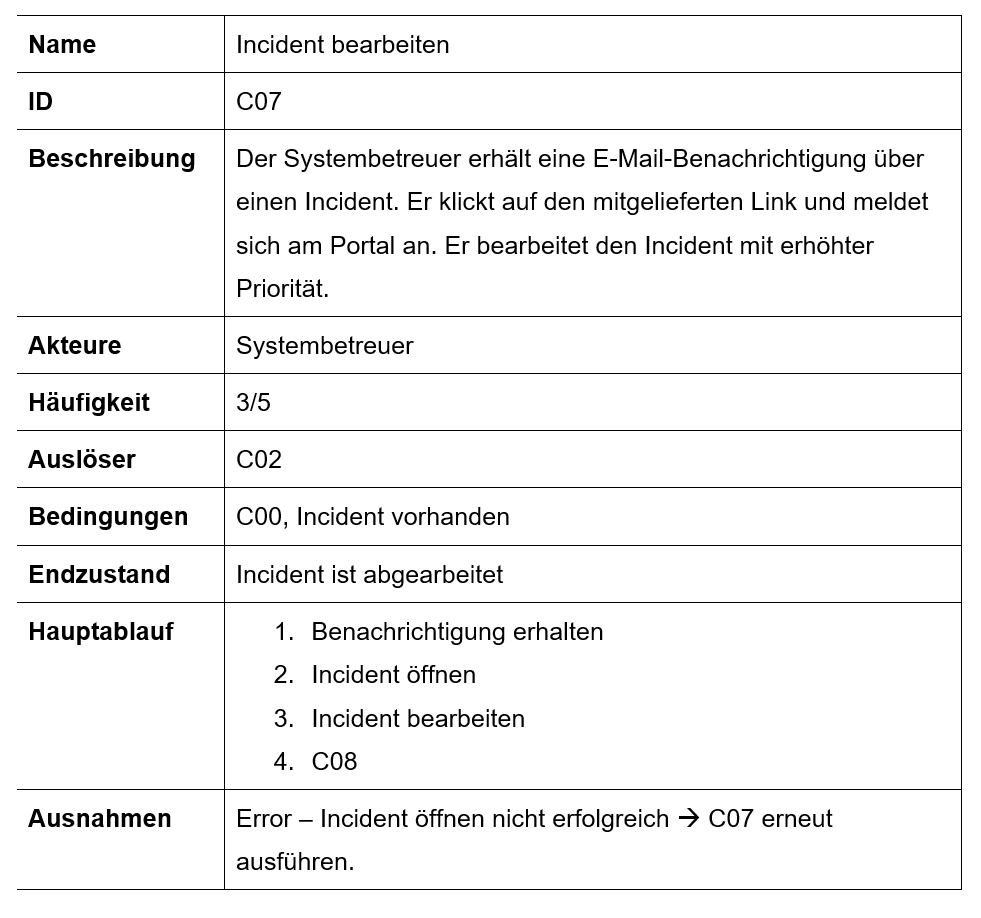
\includegraphics[scale=0.62]{figures/C07.png}
	\caption{Use-Case C07}
	\label{Abb_C07}
\end{table}

\vspace{-.5cm}	
\begin{table}[h]
	\centering
	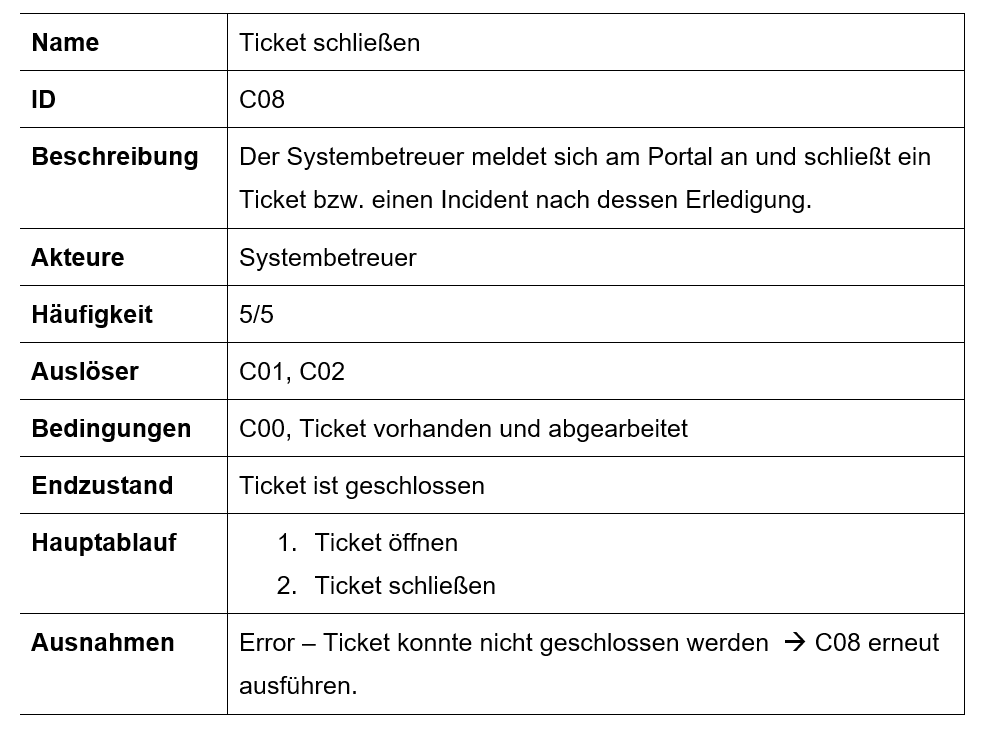
\includegraphics[scale=0.62]{figures/C08.png}
	\caption{Use-Case C08}
	\label{Abb_C08}
\end{table}


\subsection{Ablaufbeschreibung}
\textbf{C00:}
\\ 
Der Benutzer wird aufgefordert seine Benutzerdaten einzugeben.
Hat er die Daten richtig eingegeben wird er angemeldet. Sind die Daten falsch kommt er zurück zur Dateneingabe.
\\
\textbf{C01:}
\\
Der Benutzer muss zuerst ein Formular öffnen, um ein Ticket erstellen zu können. Anschließend muss das Formular ausgefüllt werden. 
\\
Nach dem Überprüfen des Tickets kann der Benutzer sich entscheiden ob er das Ticket abschickt oder ob er Änderungen vornehmen möchte. 
\\
Wenn das Abschicken fehlgeschlagen ist kommt er zum Anfang zurück. Wenn das abschicken erfolgreich war, wird das Ticket in der Datenbank gespeichert.
\\
\textbf{C02:}
\\
Der Benutzer muss zuerst ein Formular öffnen um einen Incident erstellen zu können. Anschließend muss das Formular ausgefüllt werden. Nach dem Überprüfen des Incident kann der Benutzer sich entscheiden, ob er den Incident abschickt oder ob er Änderungen vornehmen möchte.
\\
Wenn das Abschicken fehlgeschlagen ist kommt er zum Anfang zurück. Wenn das abschicken erfolgreich war wird der Incident in der Datenbank gespeichert und der Systembetreuer erhält eine Benachrichtigung.
\\
\textbf{C03:}
\\
Der Benutzer muss das Formular öffnen um den Status zu sehen. Ist das Öffnen fehlgeschlagen kommt er wieder zum Ausgangspunkt und kann es nochmal versuchen.
\\
\textbf{C04:}
\\
Um die Löschung beantragen zu können muss der Benutzer zuerst das Ticket öffnen. Danach kann er die Löschung beantragen. Schlägt dies fehl kommt er wieder zurück an den Anfang und kann es nochmal versuchen. War der Antrag auf Löschung erfolgreich erhält der Systembetreuer eine Anfrage zur Löschung.
\\
\textbf{C05:}
\\
Um ein Ticket zu löschen muss der Systembetreuer das Ticket öffnen und löschen. Schlug dies fehl kommt er wieder zurück an den Anfang und kann es nochmal versuchen. War das Löschen erfolgreich wurde das Ticket aus der Datenbank entfernt.
\\
\textbf{C06:}
\\
Um den Ticketstatus ändern zu können muss der Systembetreuer das Ticket öffnen und ändern. Schlug dies fehl kommt er wieder zurück an den Anfang und kann es nochmal versuchen. War das ändern erfolgreich wurde der Ticketstatus geändert.
\newpage
\textbf{C07:}
\\
Um ein Ticket schließen zu können muss der Systembetreuer das Ticket öffnen um es dann zu schließen. Schlug dies fehl kommt er wieder zurück an den Anfang und kann es nochmal versuchen. War das schließen erfolgreich ist das Ticket geschlossen.

\newpage
\section{Wireframes}	
\begin{figure}[h]
	\centering
	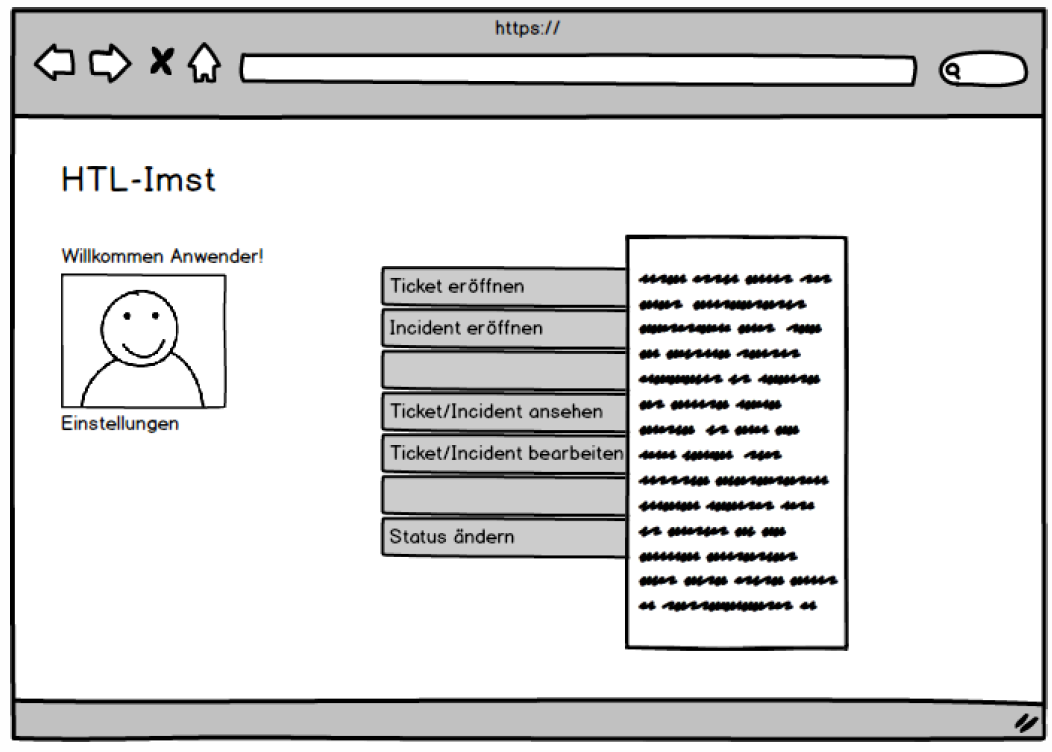
\includegraphics[scale=0.44]{figures/Wireframe_Anwender.png}
	\caption{Mockup Anwendersicht}
	\label{Abb_Mockup_Anwendersicht}
\end{figure}

\vspace{-.5cm}
\begin{figure}[h]
	\centering
	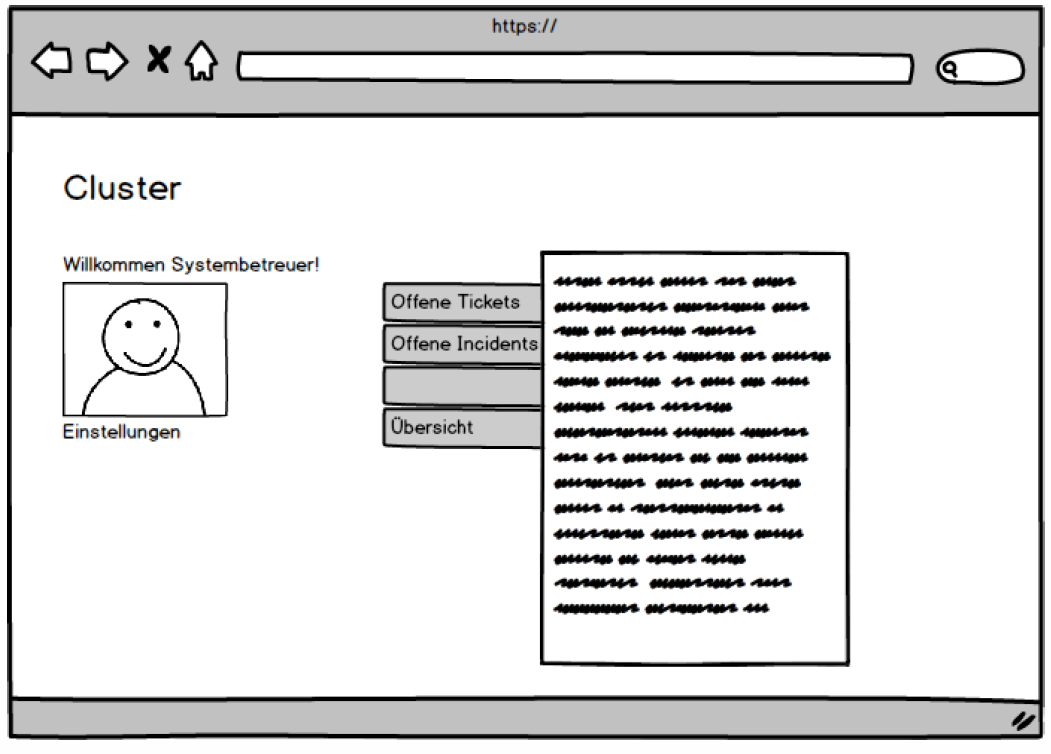
\includegraphics[scale=0.399]{figures/Wireframe_Systembetreuer.png}
	\caption{Mockup Systembetreuer}
	\label{Abb_Mockup_Systembetreuer}
\end{figure}



\vspace{.5cm}
\begin{figure}[h]
	\centering
	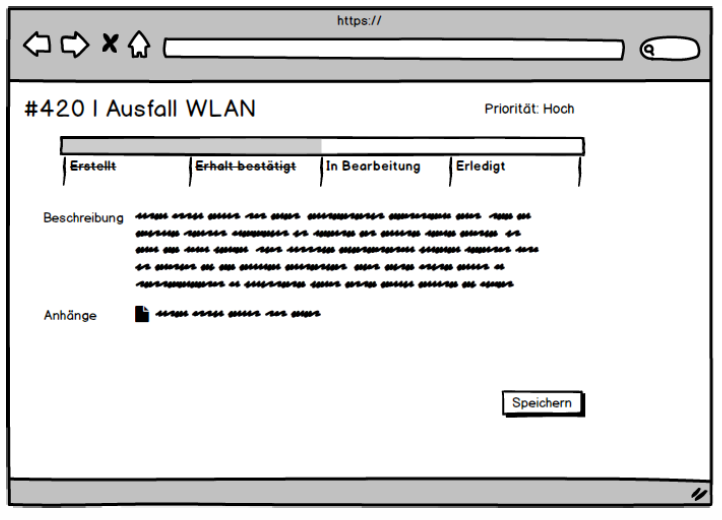
\includegraphics[scale=0.582]{figures/Wireframe_Ticket.png}
	\caption{Mockup Ticketstatus}
	\label{Abb_Mockup_Ticketstatus}
\end{figure}	

\newpage
\section{Prototyp}
\begin{figure}[h]
	\centering
	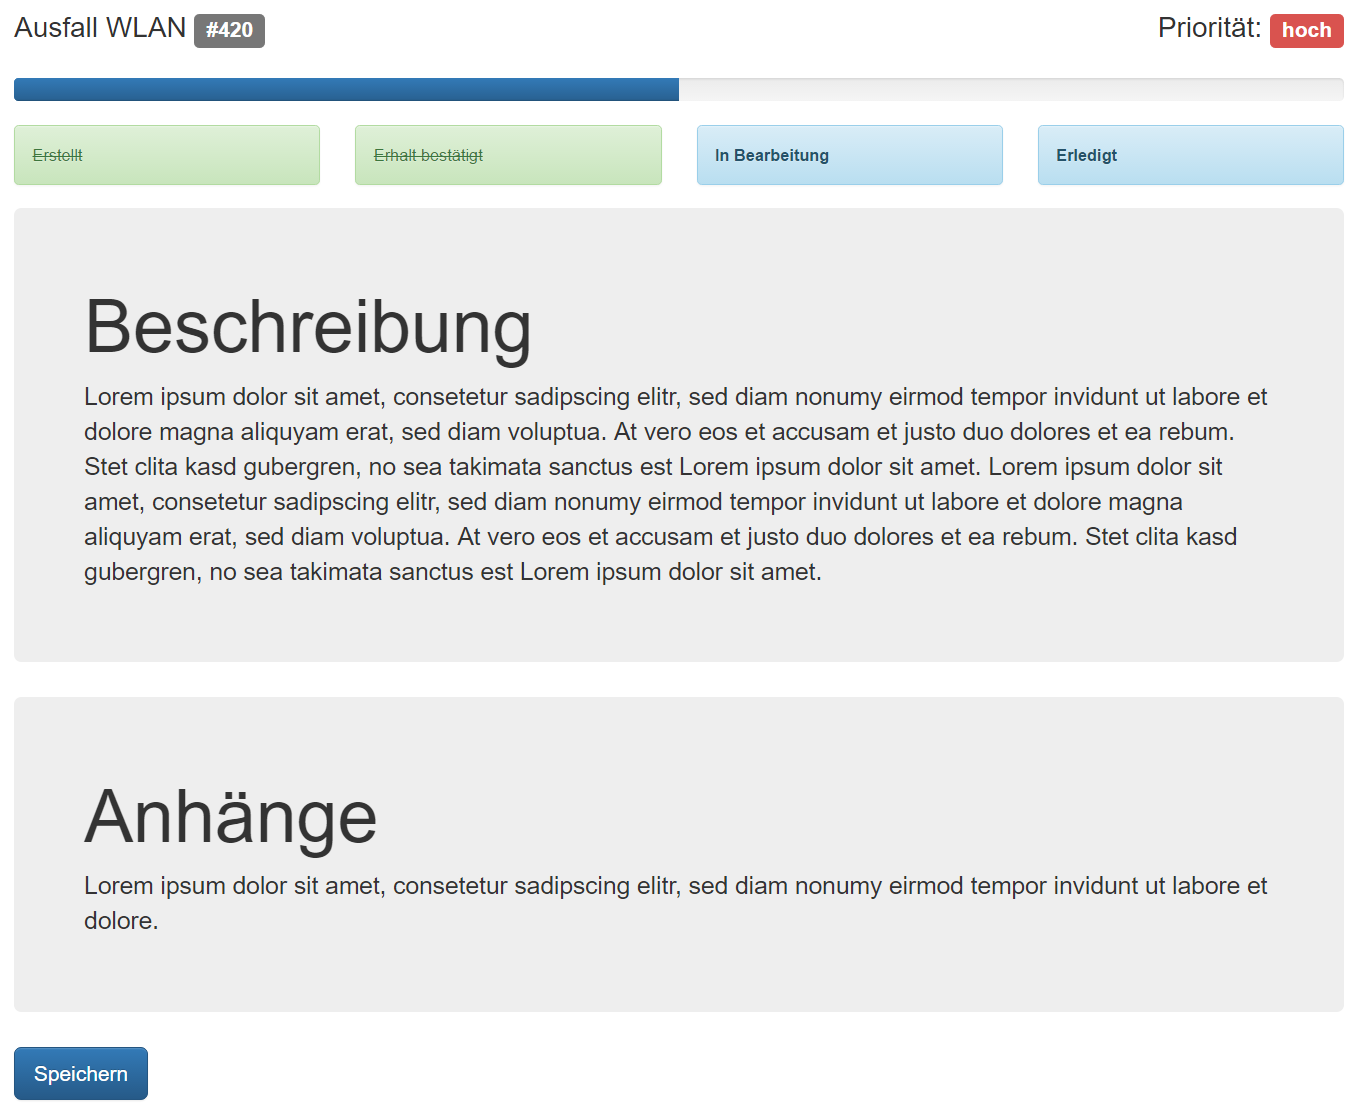
\includegraphics[scale=0.8]{figures/Prototyp.png}
	\caption{Prototyp Ticketstatus}
	\label{Abb_Prototyp_Ticketstatus}
\end{figure}


%-------------------------------------------------
%Chapter Problemanalyse Formatierungschaos bis zu diesem Punkt
%-------------------------------------------------




\newpage
\section{Domain-Class-Modelling}
\begin{itemize}
	\item "Dinge" (Rollen, Einheiten, Geräte, Events etc.) identifizieren, um die es im Projekt geht
	\item ER-Modellierung oder Klassendiagramme
	\item Zustandsdiagramme (zur Darstellung des Lebenszyklus von Domain-Klassen darstellen)
\end{itemize}

\newpage
\section{User-Interface-Design}
\begin{itemize}
	\item Mockups
	\item Wireframes
\end{itemize}


\chapter{Systementwurf Prototyp}
\def \currentAuthor{Jakob Tomasi}

Aufgrund der bereits geschilderten Umstände der Nicht Durchführbarkeit einer Adaption von \getOst\ wurde ein Prototyp für ein Ticketsystem entworfen, welcher die vom Landesschulrat und den Tiroler Schulen benötigten Funktionen mitbringt. Die Anforderungen für dieses System sind im Grunde die gleichen, welche zu Beginn an die \getOst-Adaption gestellt wurden. 
\\
Zusammengefasst sind diese:

\begin{itemize}
	\item Usability: Das System soll ohne lange Schulungsphasen oder Einlernzeit verwendet werden können. Unter Verwendung ist hauptsächlich das Absetzten von Supporttickets definiert.
	\item Mobility: Das Web-Frontend soll auch auf Smartphones und Tablets verwendet werden können und die gleichen Funktionen wie auf dem PC liefern.
	\item Adaptability: Sollten sich Anforderungen, Best Practices oder Sicherheitsanforderungen ändern, sollen diese mit so geringem Aufwand als möglich implementiert werden können.
\end{itemize}

\section{Technologie}
Für den Prototyp des Ticketsystems wurde Java Enterprise Edition ausgesucht. Diese Entscheidung basiert auf der Absicht, die bei \getOst\ gezogenen Schlüsse zu beachten und die Probleme die bei \getOst\ auftraten, zu vermeiden. JavaEE erscheint hierfür besonders geeignet, da es (in dem Verwendungsmodus, der an der Schule gelehrt wurde) von sich aus das MVC-Entwurfsmuster anwendet (mehr im nächsten Abschnitt). Des Weiteren eignet sich JavaEE für die Beseitigung der Schwächen \getOst s durch die relativ strengen Sprachkonventionen und die (beinahe) unausweichliche Objektorientierung.

\section{Architektur}
Als Basis für die Systemarchitektur wird das Model View Controller Muster verwendet. Das bedeutet die Trennung zwischen JavaBeans (Model), die direkt mit der Persistenzebene (Datenbank) arbeitet, der Benutzerschnittstelle (View; Webschicht) und der Logik (Controller; Anwendungsschicht).

%todo: Zitatquelle einfügen: Schießer, Schmollinger; Workshop Java EE 7
Das Lehrbuch fasst das Entwurfsmuster wie folgt zusammen und bringt dessen Sinn sowie Existenzberechtigung im Evaluationsprogramm \glqq Ticketsystem\grqq\ auf den Punkt:
\blockcquote[2015]{JavaEE ABC}{
Das MVC ist ein Muster, das vorgibt, wie Darstellung, Logik und Daten in einer Applikation getrennt werden sollen. Ziel dieser Trennung ist die Verbesserung der Programmstruktur und damit die Wartbarkeit, Erweiterbarkeit, und Wiederverwendbarkeit des Codes.
Das Modell kapselt die Daten und enthält je nach MVC-Ausprägung ggf. auch die fachliche Logik. Die View visualisiert das Modell und der Controller realisiert die Anwendungssteuerung Der Controller reagiert auf Benutzerinteraktionen innerhalb der View und aktualisiert ggf. die Daten am Modell. Die View wiederum passt sich je nach Ausprägung des MVC entweder automatisch an das veränderte Modell an oder wird durch den Controller über die Ausprägung informiert.
}

\begin{itemize}
	\item MVC
	\item Schichten
	\item Pipes
	\item Request Broker
	\item Service-Oriented
\end{itemize}

\section{Benutzerschnittstellen} 
Kompletter Entwurf aller Benutzerschnittstellen

\section{Datenbankentwurf}
Komplettes ER-Diagramm incl. Beschreibungen zu jeder einzelnen Tabelle und jeder Beziehung.

\section{Klassenentwurf}
Design jedes einzelnen USE-Cases

\begin{figure}[h]
	\centering
	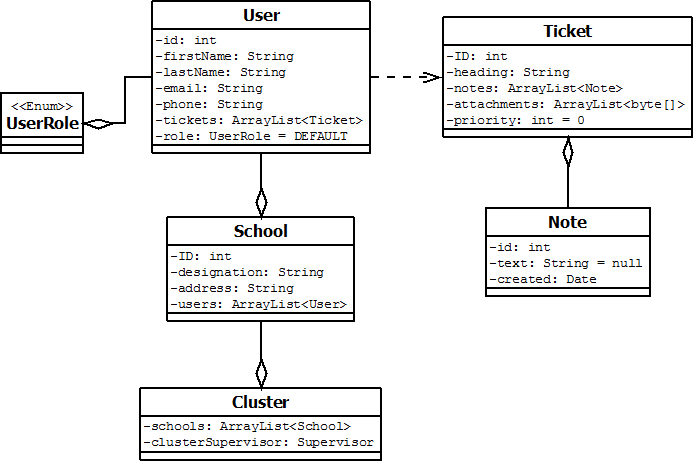
\includegraphics[scale=0.6]{figures/klassenentwurf_java_ticketsys_export.png}
	\caption{Klassenentwurf Java EE Ticketsystem}
	\label{Abb_Klassendesign_TicketSys}
\end{figure}

\begin{itemize}
	\item Design-Klassendiagramme vom Domain-Klassendiagramm ableiten (incl. detaillierter Darstellung und Verwendung von Vererbungshierarchichen, abstrakten Klassen, Interfaces)
	\item Sequenzdiagramme vom System-Sequenz-Diagramm ableiten
	\item 	Detaillierte Zustandsdiagramme für wichtige Klassen
\end{itemize}

Verwendung von CRC-Cards (Class, Responsibilities, Collaboration) für die Klassen
\begin{itemize}
	\item um Verantwortlichkeiten und Zusammenarbeit zwischen Klassen zu definieren und
	\item um auf den Entwurf der Geschäftslogik zu fokussieren
\end{itemize}

Design-Klassen für jeden einzelnen USE-Case können sein:
\begin{itemize}
	\item UI-Klassen
	\item Data-Access-Klassen
	\item Entity-Klassen (Domain-Klassen)
	\item Controller-Klassen
	\item Business-Logik-Klassen
	\item View-Klassen
\end{itemize}

Optimierung des Entwurfs (Modularisierung, Erweiterbarkeit, Lesbarkeit):
\begin{itemize}
	\item Kopplung optimieren
	\item 	Kohäsion optimieren
	\item 	SOLID
	\item 	Entwurfsmuster einsetzen
\end{itemize}

\section{Sicherheit des Systems}
Beschreibung aller sicherheitsrelevanten Designentscheidungen;

\chapter{Implementierung}
Detaillierte Beschreibung der Implementierung aller Teilkomponenten der Software entlang der zentralsten Use-Cases:

\begin{itemize}
	\item GUI-Implementierung
	\item Controllerlogik
	\item Geschäftslogik
	\item Datenbankzugriffe
\end{itemize}

Detaillierte Beschreibung der Teststrategie (Testdriven Development):

\begin{itemize}
	\item UNIT-Tests (Funktional)
	\item Integrationstests
\end{itemize}

Zu Codesequenzen:
\begin{itemize}
	\item kurze Codesequenzen direkt im Text (mit Zeilnnummern auf die man in der Beschreibung verweisen kann)
	\item lange Codesequenzen in den Anhang (mit Zeilennummer) und darauf verweisen (wie z.B. hier \cref{qj})
\end{itemize}

\chapter{Deployment}
\begin{itemize}
	\item Design der Ausführungsumgebung (Produktivenvironment)
	\item Umsetzung der Ausführungsumgebung
	\item Deployment
	\item DevOps-Thema
\end{itemize}

\chapter{Tests}

%todo: Testfälle doch in diesem Chapter verwenden?!? Vorlage etwas unklar
\section{Systemtests} 
Systemtests aller implementierten Funktionalitäten lt. Pflichtenheft
\begin{itemize}
	\item Beschreibung der Teststrategie
	\item Testfall 1
	\item Testfall 2
	\item Tesfall 3
	\item …
\end{itemize}

\section{Akzeptanztests}

\chapter{Projektevaluation}
siehe Projektmanagement-Unterricht

\chapter{Benutzerhandbuch} 
falls im Projekt gefordert

\chapter{Zusammenfassung}
\begin{itemize}
	\item Etwas längere Form des Abstracts
	\item Detaillierte Beschreibung des Outputs der Arbeit
\end{itemize}